\section{Introduction}
\label{sec:intro}

\begin{figure}[!t]
	\centering
	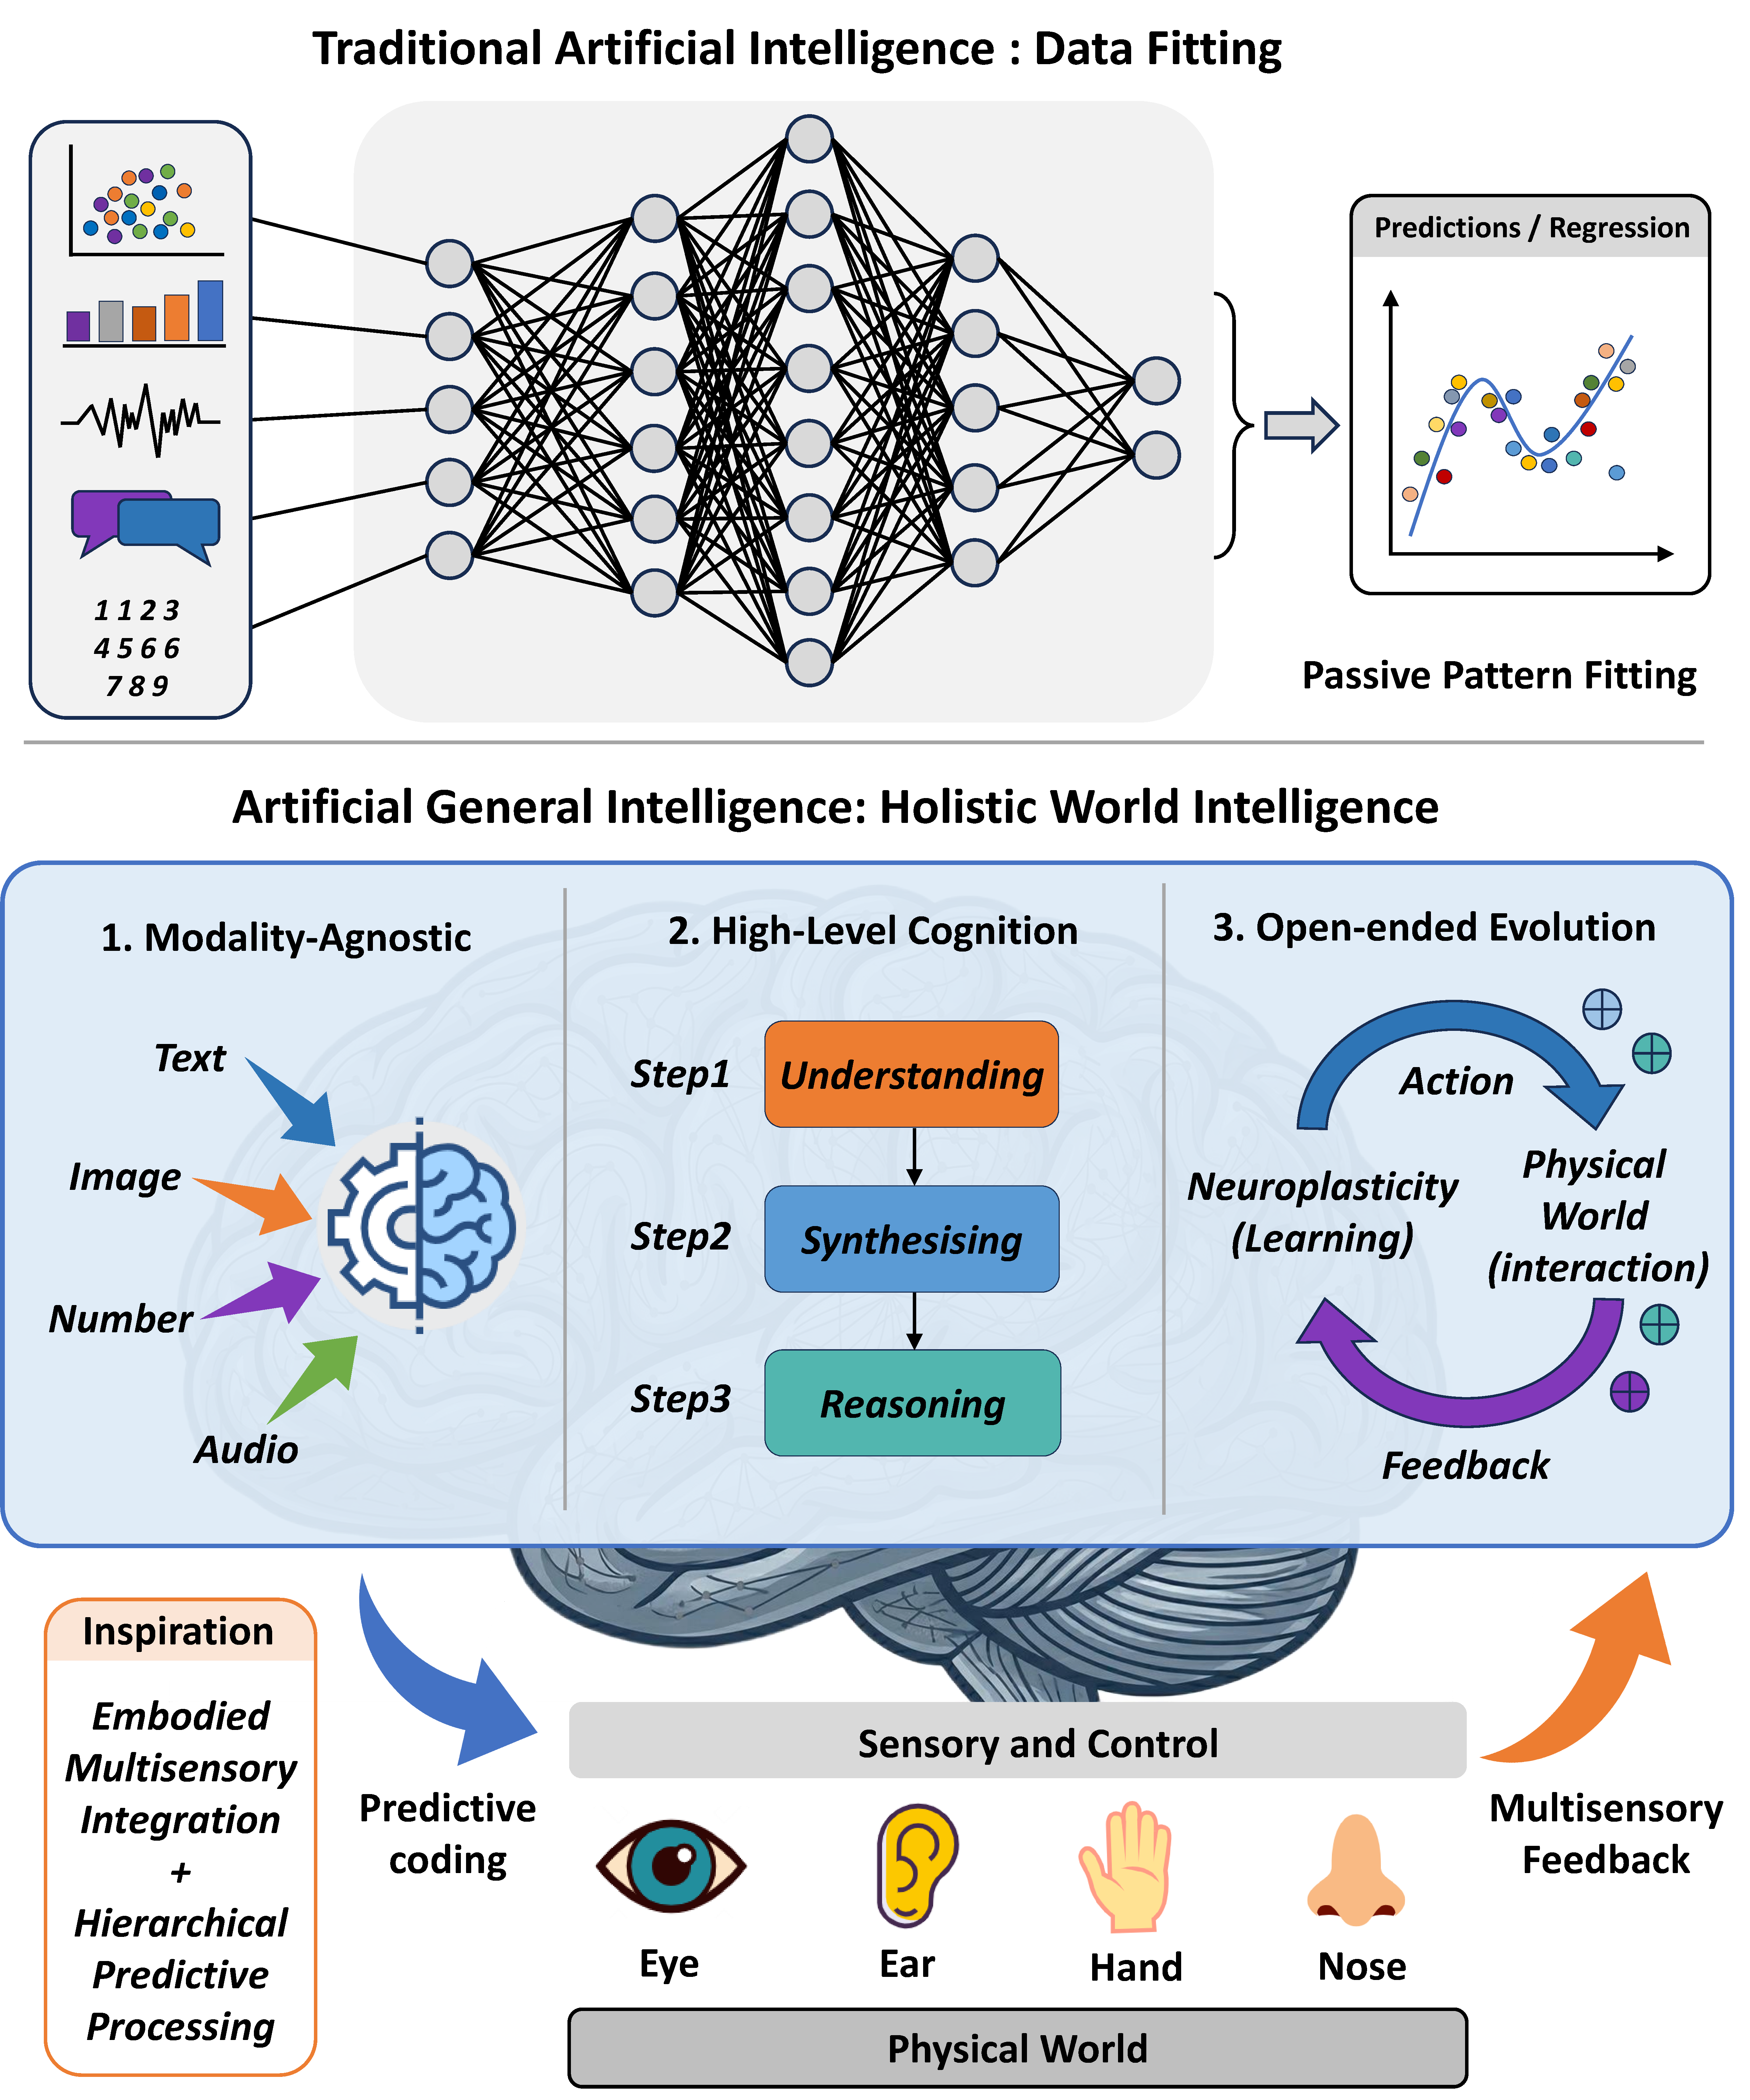
\includegraphics[scale=0.1]{figure/figure22.pdf}
    \vspace{-3mm}
	\caption{The Paradigm Shift from Traditional Statistical Data Fitting to Holistic World Intelligence (HWI) for AGI. }
    \vspace{-5mm}
	\label{figure1}
\end{figure}

\begin{figure*}[!t]
	\centering
	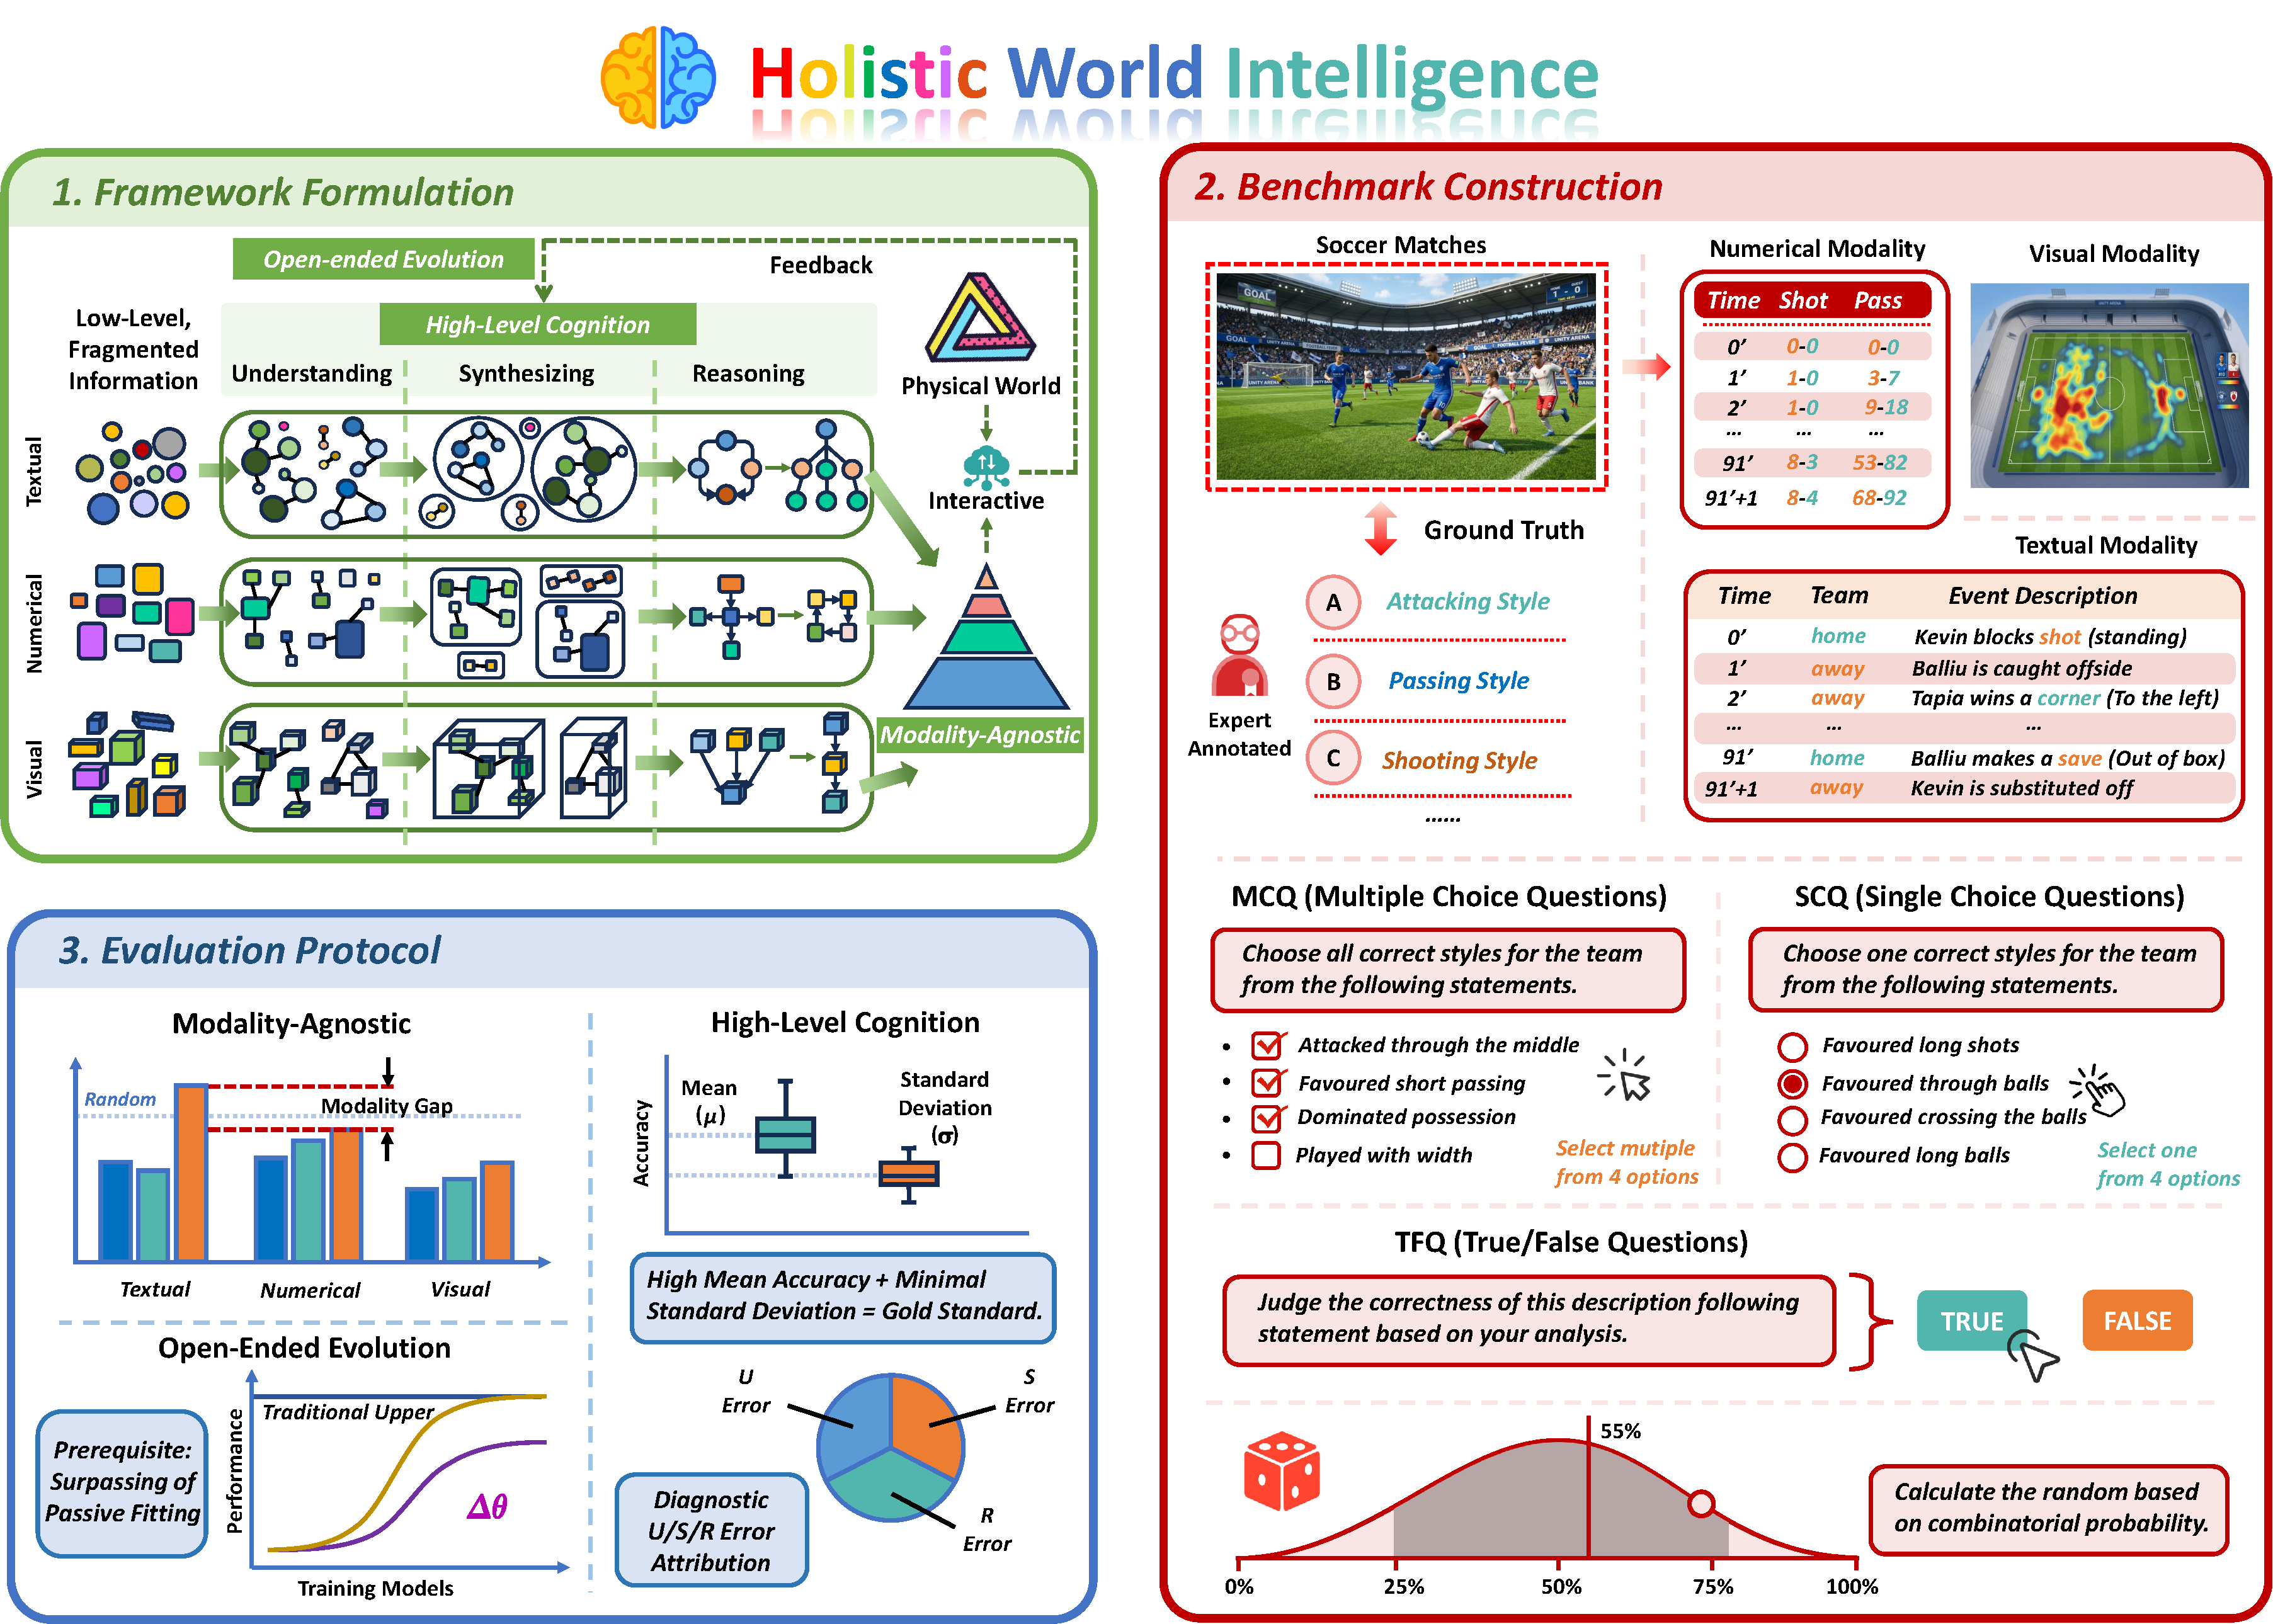
\includegraphics[scale=0.29]{figure/figure2.pdf}
    \vspace{-2mm}
	\caption{The Systematic Paradigm for Evaluating Holistic World Intelligence (HWI) across Multi-modal Representations. }
    \vspace{-3mm}
	\label{figure2}
\end{figure*}

The inherent complexity and heterogeneity of the physical world pose a fundamental bottleneck to the evolution toward Artificial General Intelligence (AGI) \cite{goertzel2014artificial}.
This reality subjects Large Language Models (LLMs), the quintessential paradigm in the pursuit of AGI \cite{bubeck2023paper}, to foundational performance scrutiny \cite{zhao2023survey}.
Profoundly, addressing this bottleneck necessitates a paradigm shift toward \textbf{Holistic World Intelligence} (HWI), an endogenously and perpetually integrated capacity to process heterogeneous real-world representations.
Inspired by cognitive neuroscience represented by Embodied Multisensory Integration \cite{stein2008multisensory} and Hierarchical Predictive Processing \cite{clark2013whatever}, we posit that HWI can be anchored to three core attributes conceptually illustrated in Figure~\ref{figure1}.
First, HWI is inherently \emph{Modality-Agnostic}, enabling the resolution of heterogeneous physical scenarios through unified internal representations that transcend disparate sensory boundaries \cite{ngiam2011multimodal}.
Second, it embodies \emph{High-Level Cognition} (HLC), mimicking the human-like cognitive hierarchy to integrate foundational functions into structured reasoning chains \cite{laird2017standard, bengio2017consciousness}.
Third, it facilitates \emph{Open-ended Evolution}, a neuroplasticity-inspired attribute \cite{hassabis2017neuroscience} that empowers the model to continuously and actively augment its capabilities through autonomous environmental interaction \cite{silver2021reward}.

Despite their prevalence, current approaches fail to internalize these core attributes of HWI.
Predominantly, while attempting to bridge heterogeneity gaps, Multimodal Large Language Models (MLLMs) largely rely on superficial semantic alignment \cite{radford2021learning} rather than achieving a truly Modality-Agnostic unified representation, leaving them fragmented when facing multidimensional physical properties \cite{wu2024next, tong2024eyes}.
Simultaneously, prevailing reasoning paradigms often focus on scaling exogenous logical complexity via externally designed heuristics \cite{wei2022chain, yao2023tree}; however, such plug-and-play enhancements do not translate into genuine endogenous reasoning capabilities or autonomous cognitive depth \cite{huang2023large}.
Most critically, the current framework still remains restricted to modeling the static physical world through passive data-fitting \cite{kaplan2020scaling}, rather than actively exploring and exploiting dynamic environmental feedback to foster sustained, open-ended cognitive growth \cite{wang2023voyager}.
Consequently, these gaps jointly raise a fundamental question: \emph{Can a unified architecture truly internalize the holistic laws of the physical world to attain authentic, world-level intelligence?}

Fundamentally, overcoming these persistent bottlenecks is currently hindered by systemic deficiencies across three critical dimensions.
\emph{Architecturally}, the absence of established HWI-centric datasets and evaluation benchmarks \cite{srivastava2022behavior, gu2023maniskill2} precludes a rigorous and empirical measurement of holistic world representations.
\emph{Theoretically}, a lack of principled analytical guidance consigns the internal mechanisms of world-level cognition to a black box \cite{li2022emergent}, rendering the emergence of HWI largely uninterpretable and opaque \cite{nanda2023progress}.
\emph{Methodologically}, the dearth of novel paradigms capable of triggering endogenous logical growth and continuous environmental interaction prevents a substantive transition from static fitting to active intelligence augmentation \cite{park2023generative}.
To address these multifaceted gaps, this work establishes a structured framework to rigorously analyze the three defining attributes of HWI, providing both theoretical insights and empirical evidence to guide the development of future effective AGI methodologies \cite{bengio2021deep}.

Therefore, this work establishes a holistic and principled evaluation paradigm to bridge the existing gaps between current LLMs and the realization of authentic AGI \cite{mahowald2024dissociating}. Our specific contributions are summarized across three dimensions:
\begin{itemize}[leftmargin=*]
\item \textbf{Systematic Framework and Infrastructure:} We propose a comprehensive framework for \textbf{Holistic World Intelligence}, providing a formal definition of its core attributes (Sec.~\ref{formulation}). To enable empirical measurement, we introduce a specialized benchmark named \textbf{WorldScope} (Sec.~\ref{benchmark}) and a rigorous evaluation protocol (Sec.~\ref{protocol}) to assess the emergence of this capability under heterogeneous real-world representations.
\item \textbf{Empirical Investigation of Capability Collapse:} We conduct an extensive empirical study revealing a critical phenomenon we term \emph{Capability Collapse} in current state-of-the-art multimodal models when processing complex physical data (Sec.~\ref{phenomenon}). By delving into the underlying causes of this failure, we provide a foundational analysis that fills the current void in systematic understanding of world-level performance (Sec.~\ref{analysis}).
\item \textbf{In-depth Analysis and Future Roadmap:} We perform a granular investigation into three pillars of HWI: \emph{Modality-Agnosticism} (Sec.~\ref{modality}), \emph{High-level Cognition} (Sec.~\ref{HLC}), and \emph{Open-ended Evolution} (Sec.~\ref{evolution}). Based on these insights, we propose preliminary improvements and offer a strategic roadmap to guide future efforts toward AGI through LLMs (Sec.~\ref{future}).
\end{itemize}
